\section{The corpus}
\begin{wrapfigure}{r}{0.5\textwidth}
    \centering
    \fbox{
\includegraphics[width=0.3\textwidth]{media/official1.png}}
    \caption{
        The position of an `official homepage' link on a Wikipedia
        webpage's {\tt vcard} (highlighted in yellow).
        \label{official1}
    }
\end{wrapfigure}
As will be discussed in Section \ref{corpus}, the unstructured web
poses a challenge to structured data extraction. In Figures
\ref{official1} and \ref{official2}, three different
positions for `official homepage' links appear on
newspapers' Wikipedia articles.  An intelligent web scraper is
needed, capable of recognising all different scenarios, and extracting
the links most likely to represent official homepages.

Another task arises after the official homepages for news sources
are determined.  Which links on a homepage or other
index page correspond to news items and other news indices?
(Figures \ref{index1} and \ref{index2})

\begin{figure}[H]
    \centering
    \fbox{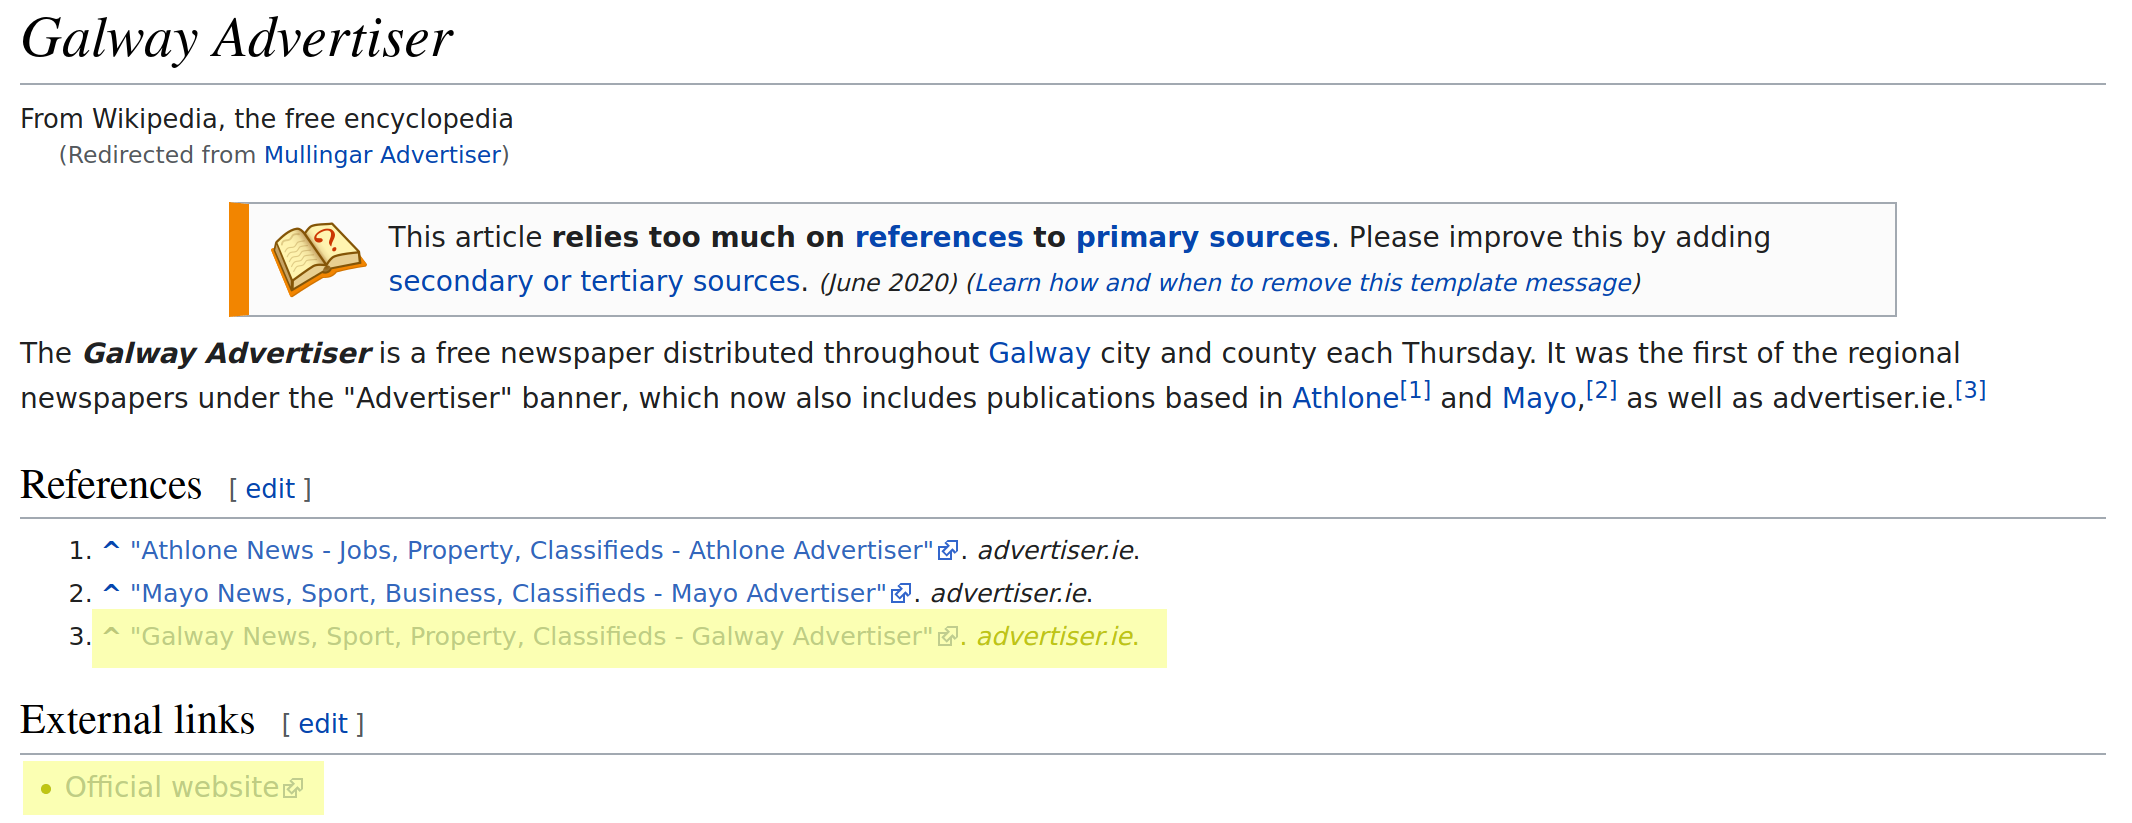
\includegraphics[width=0.8\textwidth]{media/official2.png}}
    \caption{
        \raggedright
        The position of official homepage links at the bottom
        of another Wikipedia webpage.\label{official2}
    }
\end{figure}
\begin{figure}[H]
    \centering
    \fbox{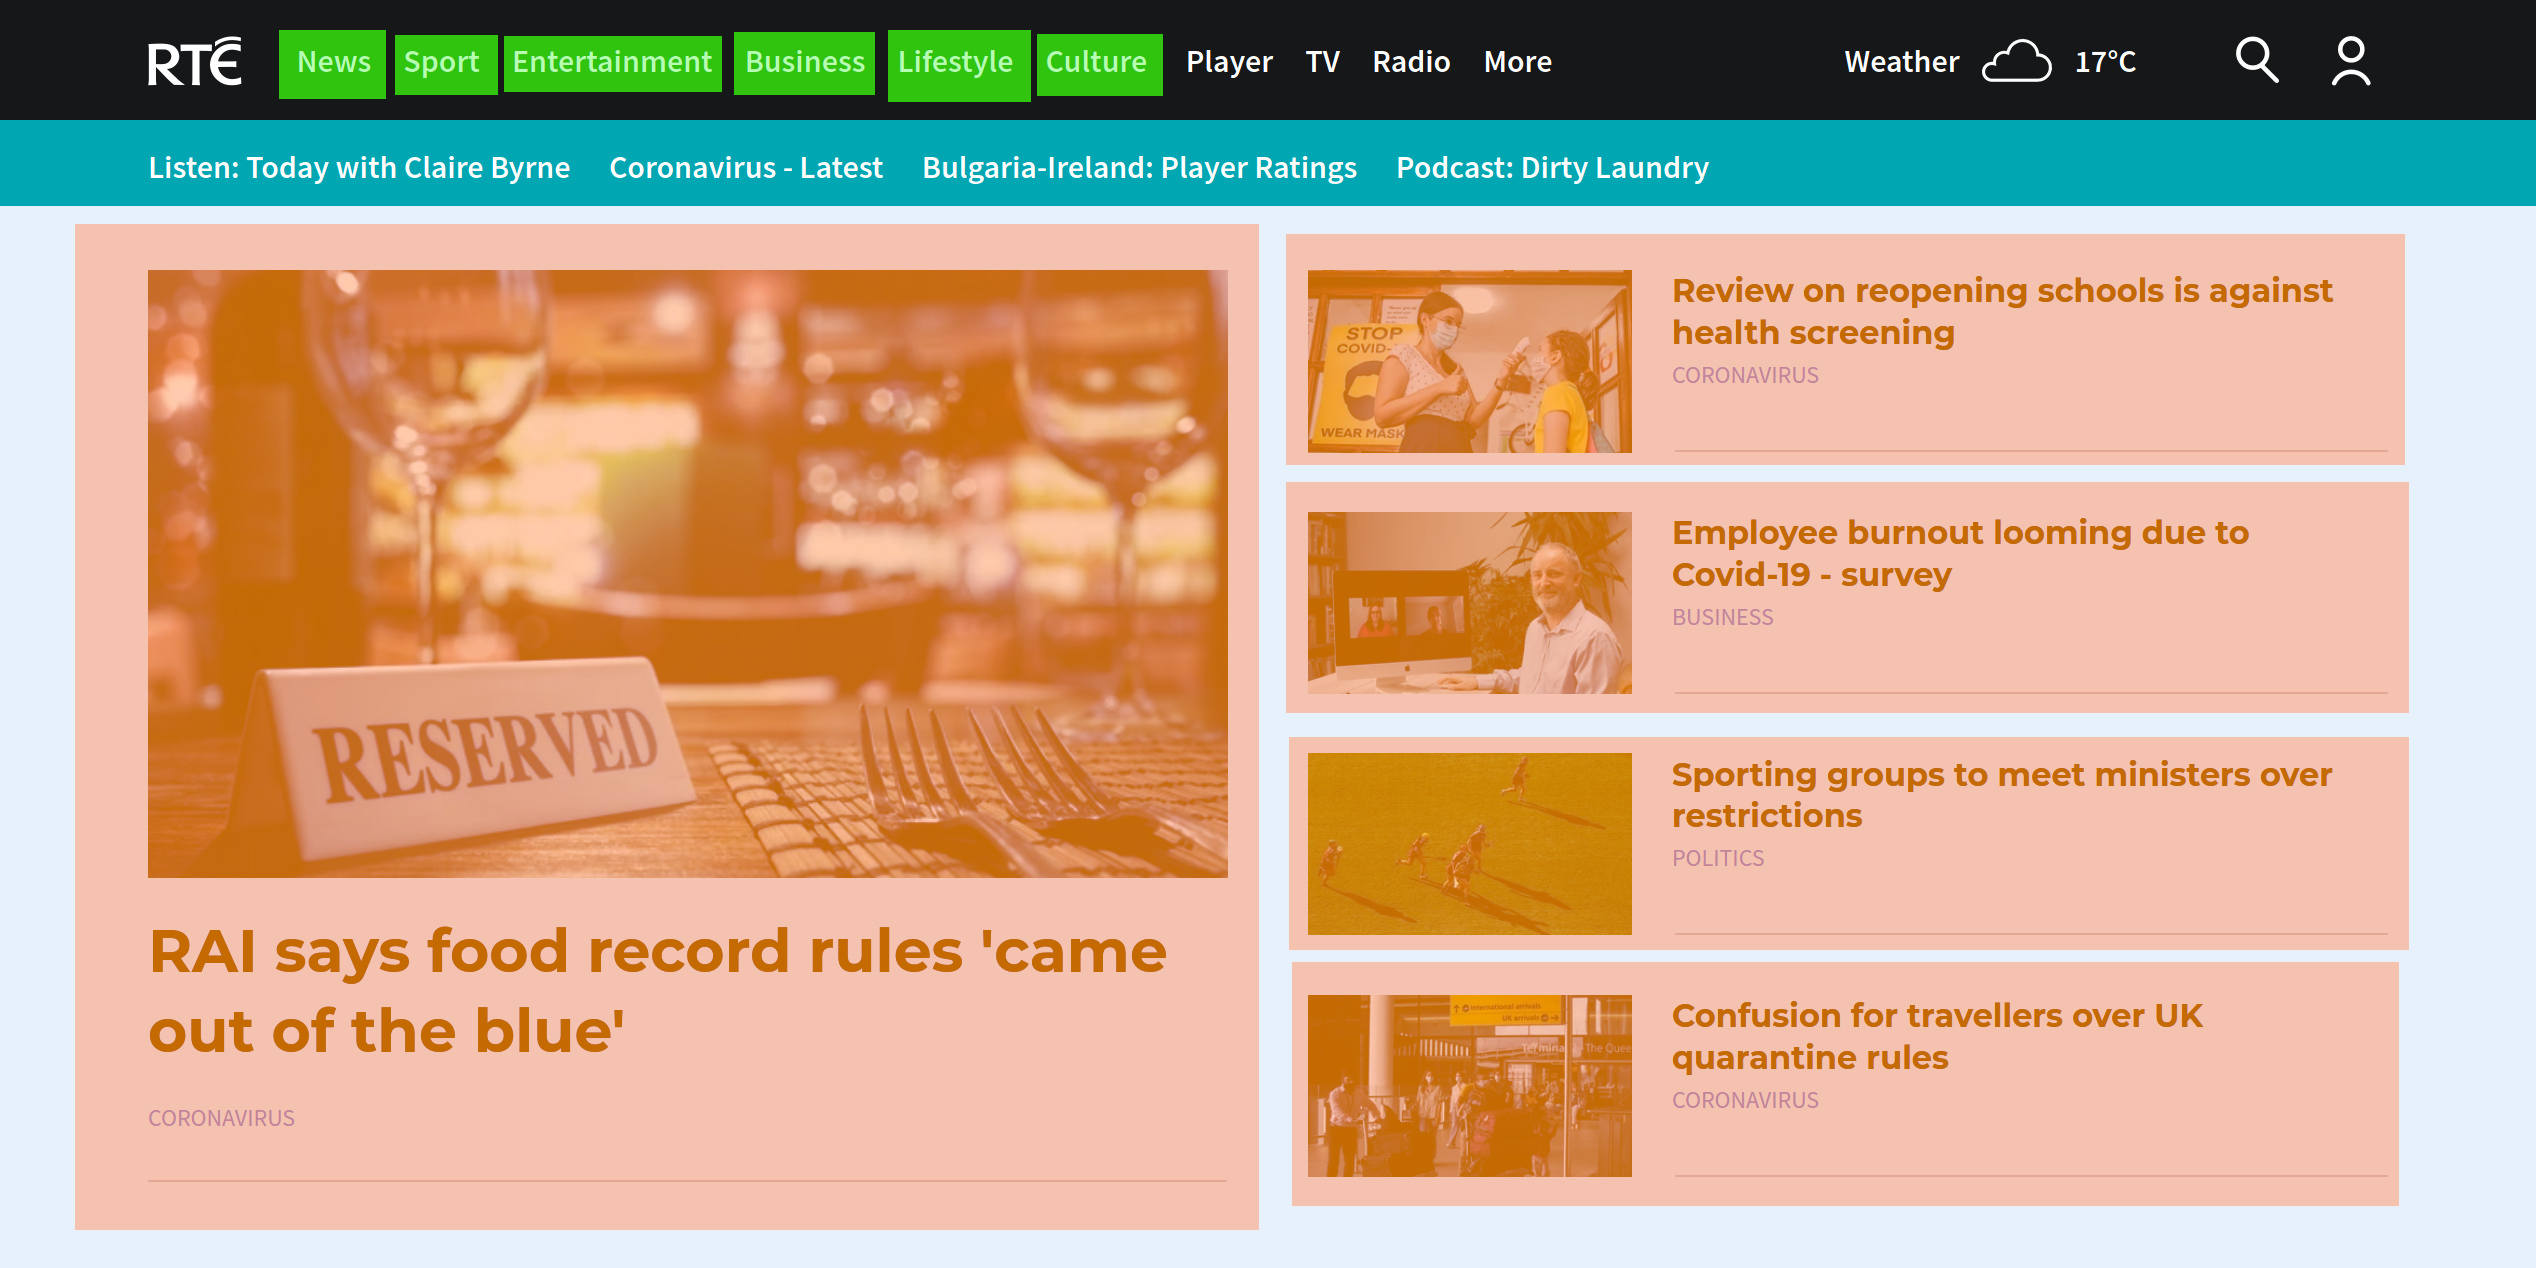
\includegraphics[width=0.8\textwidth]{media/index.png}}
    \caption{
        Index links (green) and item links (orange)
        on the RTE homepage.\label{index1}
    }
\end{figure}
\begin{figure}[H]
    \centering
    \fbox{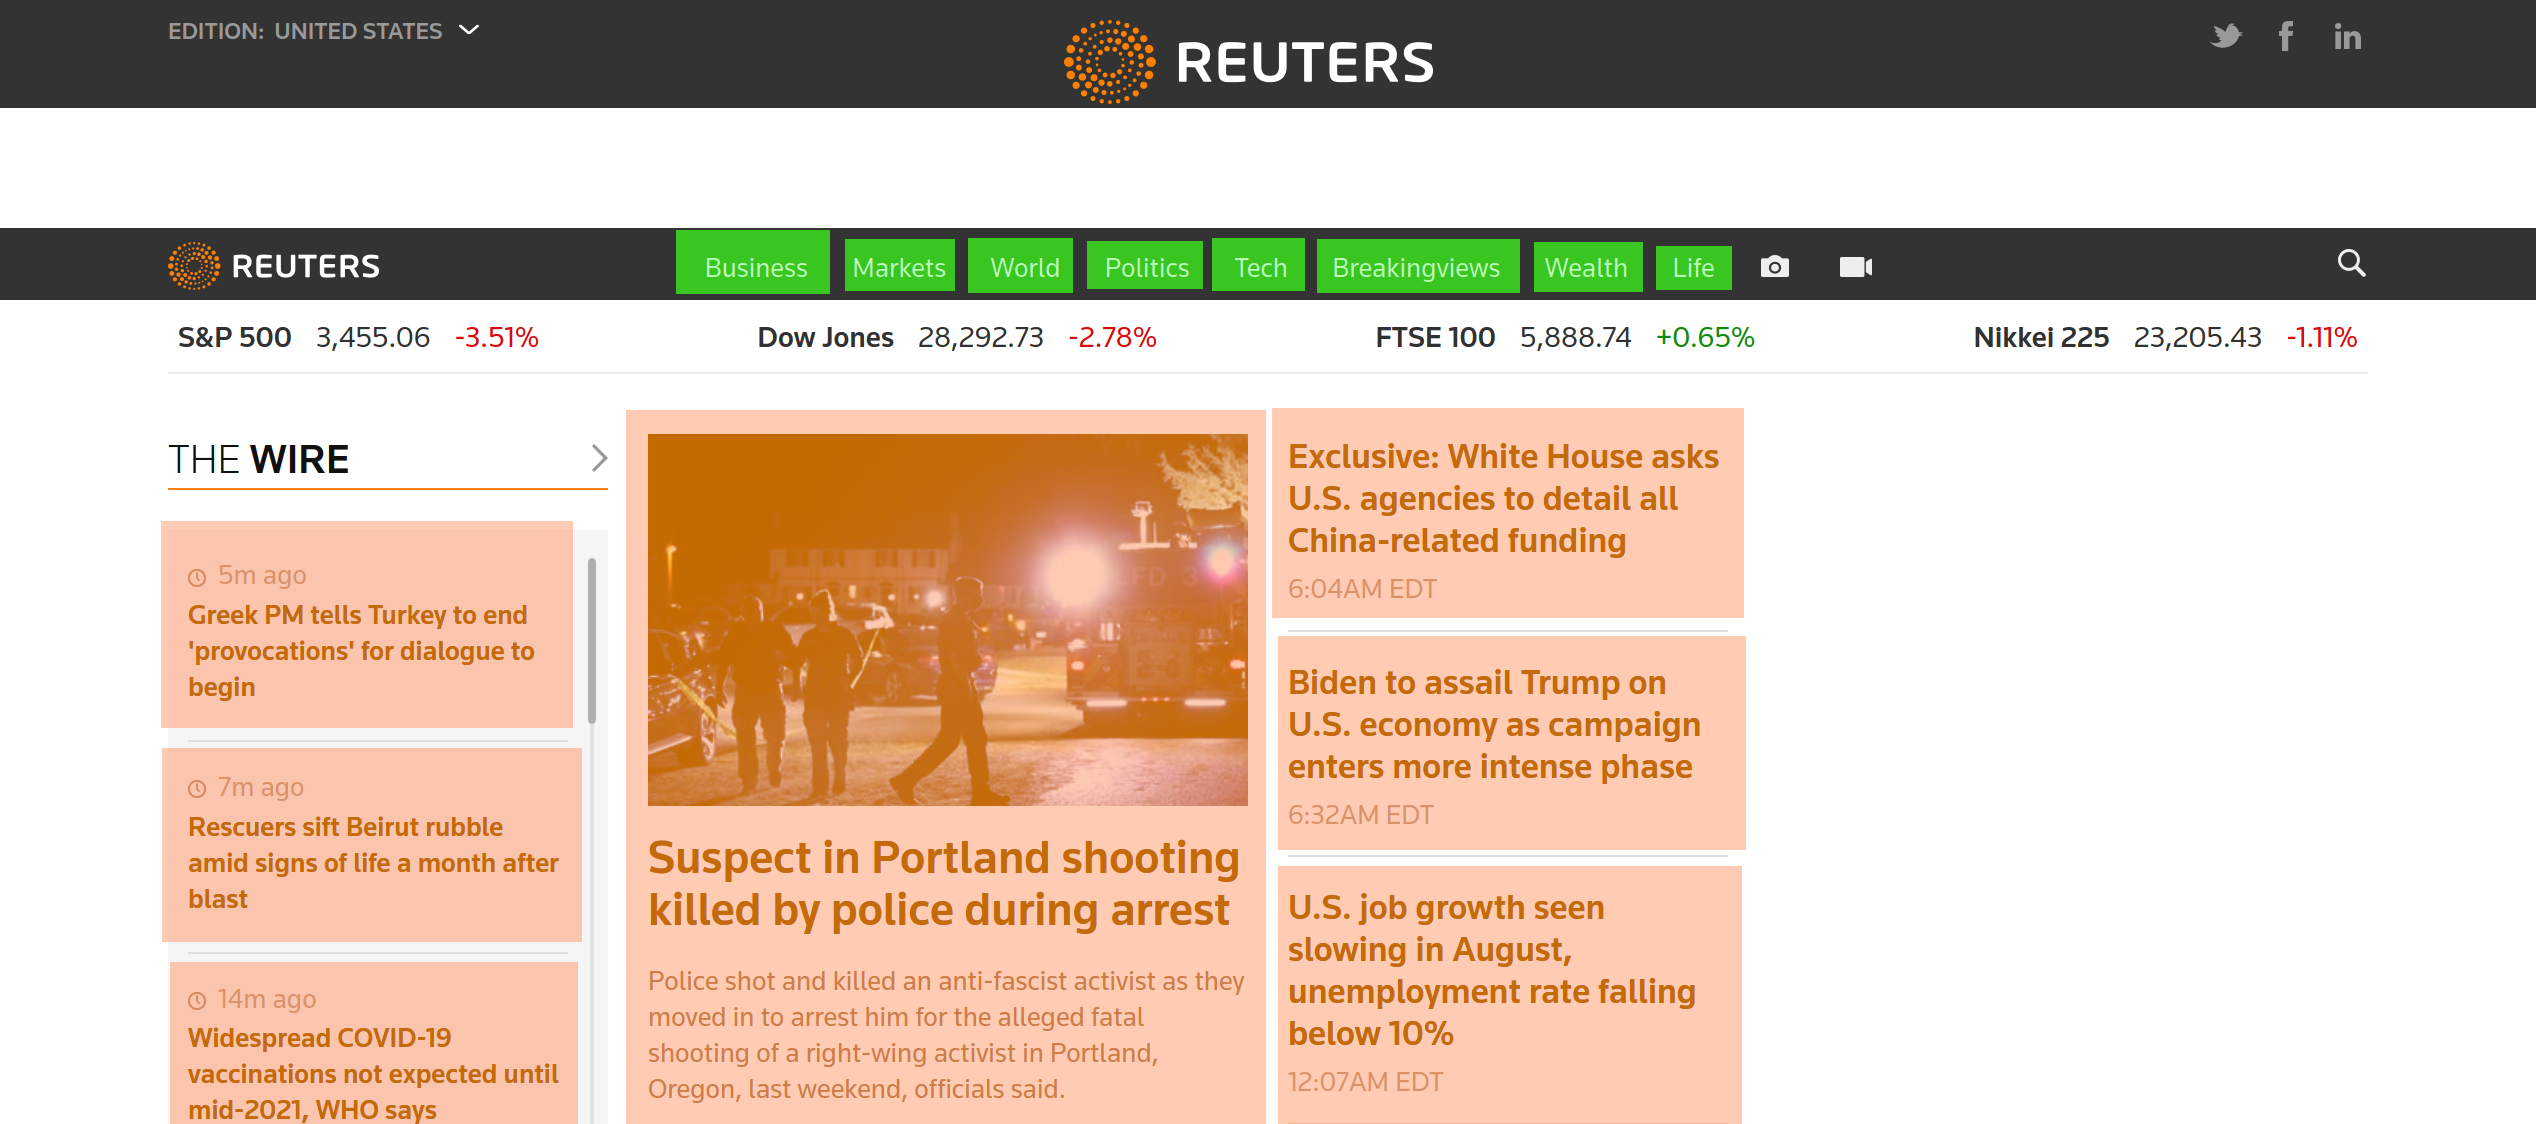
\includegraphics[width=0.8\textwidth]{media/index2.png}}
    \caption{
        Index links (green) and item links (orange)
        on the Reuters homepage.\label{index2}
    }
\end{figure}\clearpage

Within news items on each page, there are several more relation
extraction tasks.  Figures \ref{item1} and \ref{item2} show some of
the key labelled information associated with news items.  Note that
in one news item (\ref{item1}), there is a single author, and in the
other there are two authors (\ref{item2}).  The publication date is
labelled relatively in one news item, ``a day ago'', and literally
in the other news item.  One news item has a byline, the other one
doesn't.
\begin{figure}[H]
    \centering
    \fbox{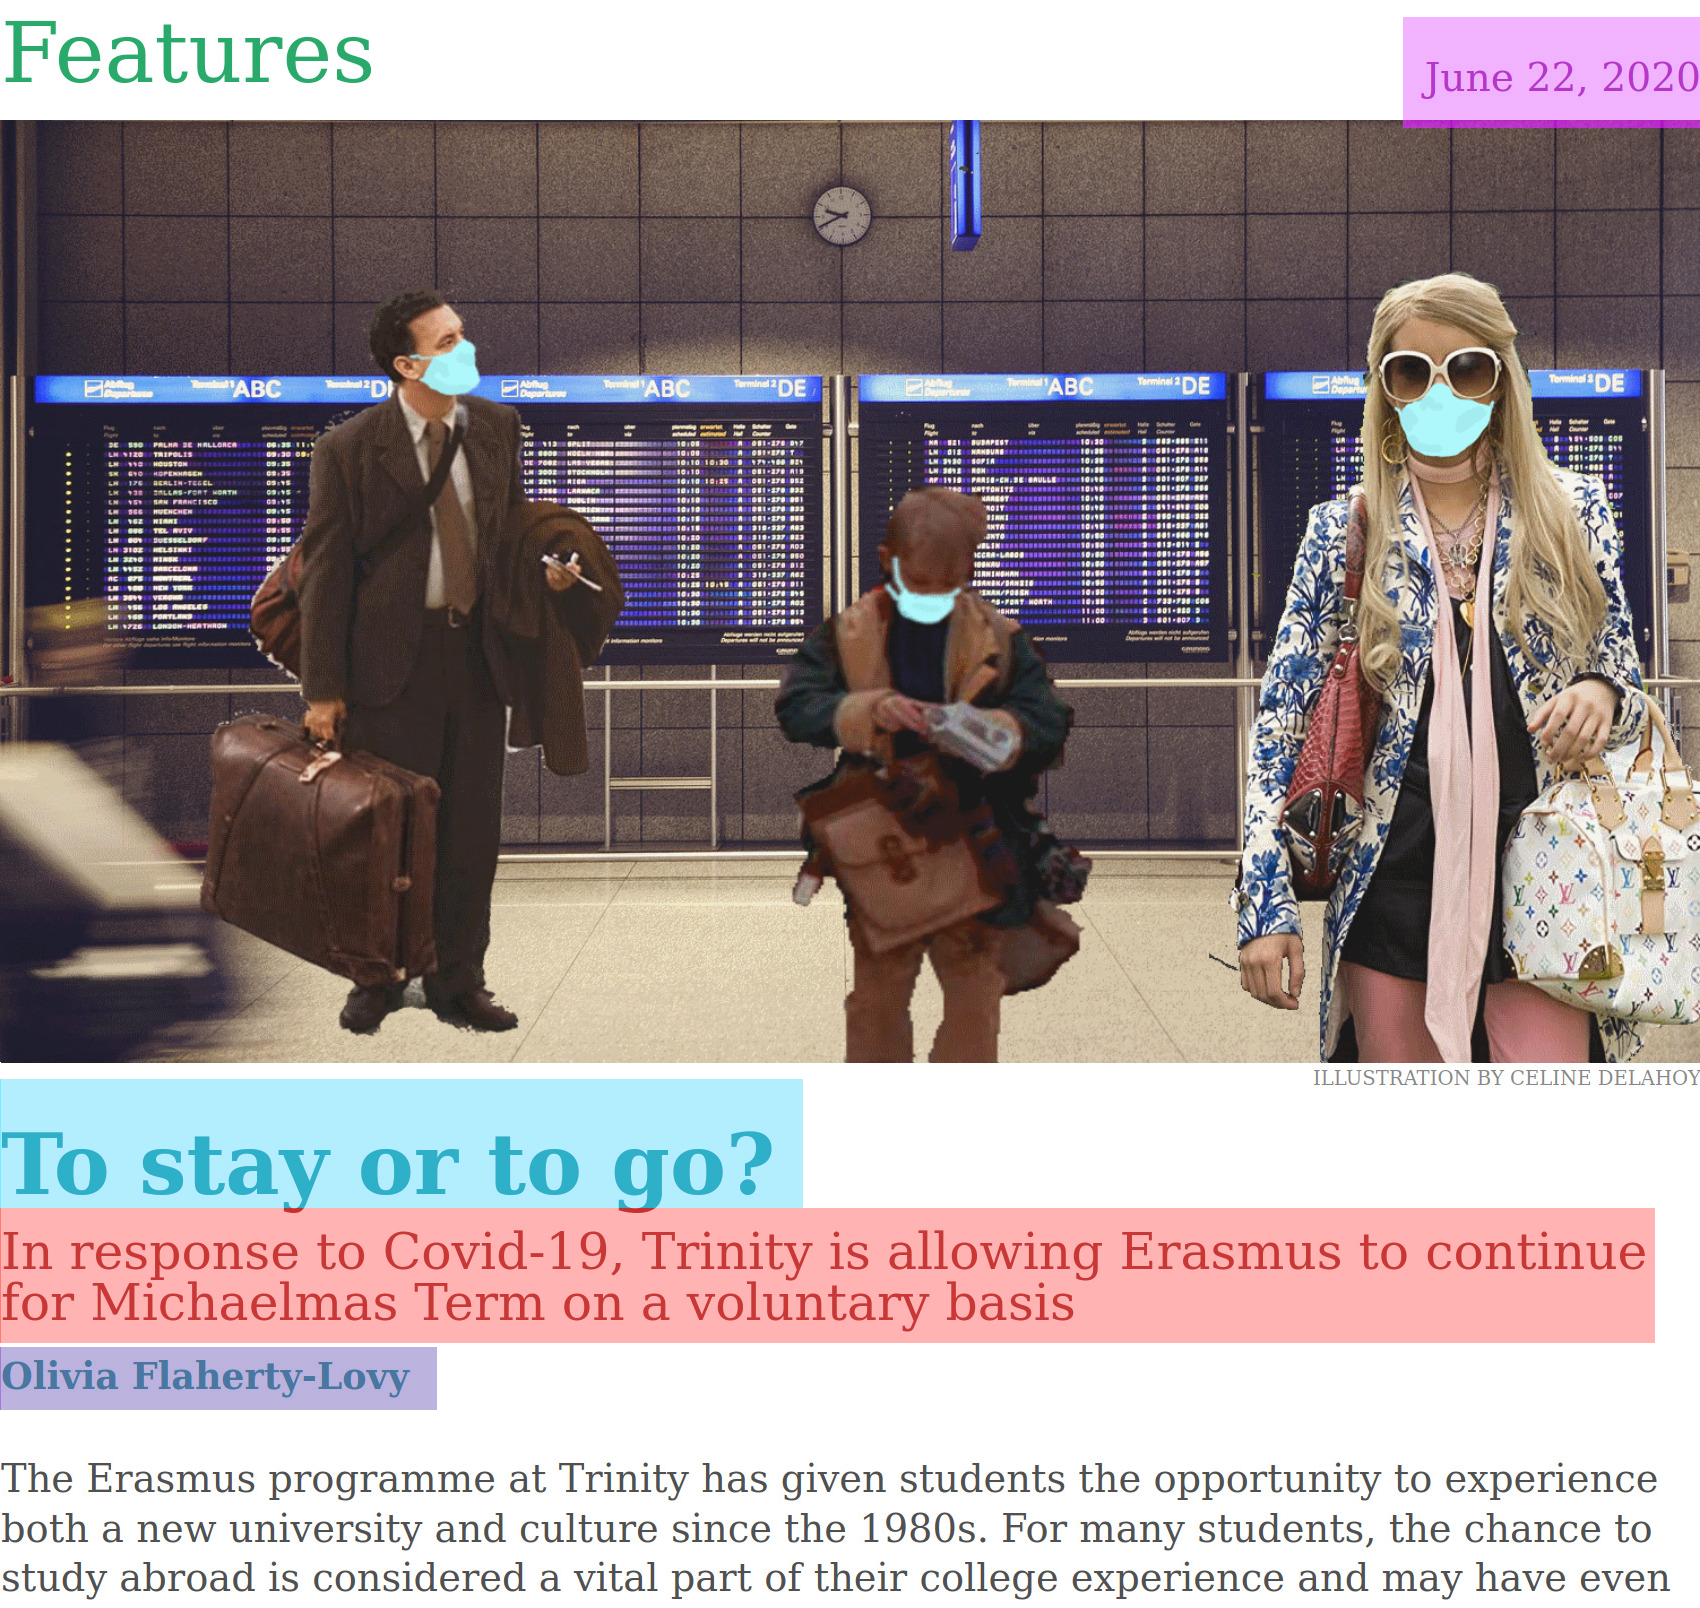
\includegraphics[width=0.7\textwidth]{media/item1.png}}
    \caption{Information of interest on a news item page:
    publication date (pink), headline (blue), byline (red),
    author name (purple).\label{item1}
    }
\end{figure}
\begin{figure}[H]
    \centering
    \fbox{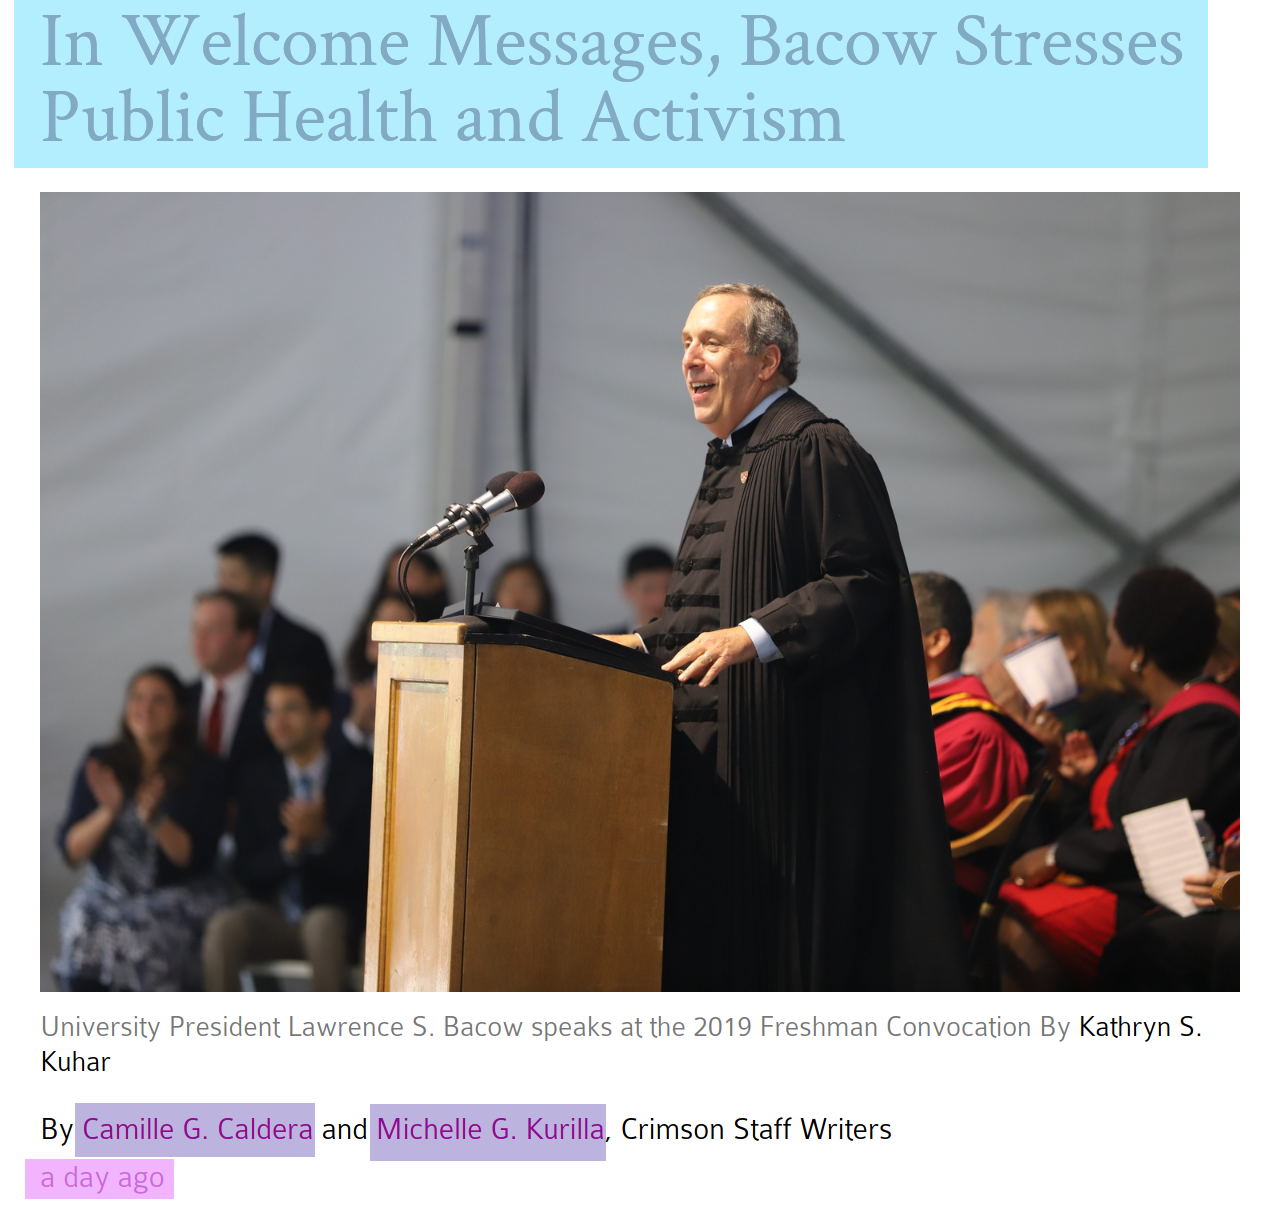
\includegraphics[width=0.7\textwidth]{media/item2.png}}
    \caption{The same information types from Figure \ref{item1},
    on a different news item page.\label{item2}}
\end{figure}
\noindent The underlying {\tt HTML} for each of these webpages
also varies greatly.  This level of variance necessitates
a dynamic, probabalistic approach to web scraping, rather than
manually writing rules based on the assumption of semantically
correct and uniform {\tt HTML}.

With a firm grasp on the tasks, terminology, and the structure the
dataset will take, the next chapter will cover background research
related to these tasks.